% Supplement after the typed SourceFigure explanation. Requires graphicx/tikz.
\begin{center}
\begin{minipage}[t]{.46\linewidth}\vspace{0pt}\centering
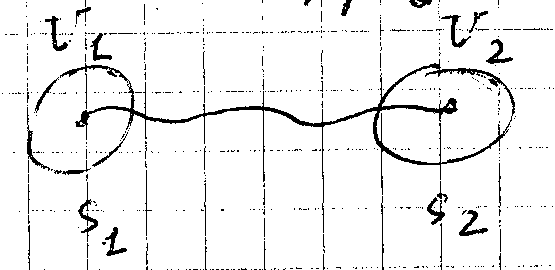
\includegraphics[width=\linewidth]{figures/gelfand-0151-p001386-path-original.png}\par\smallskip
{\footnotesize Original manuscript detail: \texttt{GELFAND-P001386}}
\end{minipage}\hfill
\begin{minipage}[t]{.50\linewidth}\vspace{0pt}\centering
{\footnotesize Partial typographic recreation}\par\smallskip
% Partial native recreation of GELFAND-P001386. No transport arrow is supplied.
% Preserve the visible break in the left oval; bottom labels remain candidates.
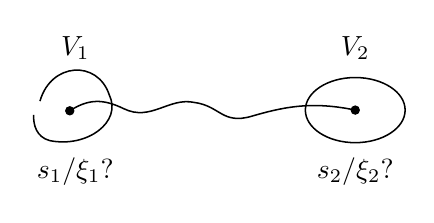
\begin{tikzpicture}[x=.88cm,y=.88cm,line width=.55pt]
\draw (-.43,.14) .. controls (-.27,.70) and (.40,.74) .. (.57,.23)
  .. controls (.76,-.16) and (.25,-.54) .. (-.29,-.43)
  .. controls (-.48,-.38) and (-.53,-.20) .. (-.52,-.06);
\draw (4.12,.01) ellipse (.72 and .47);
\draw (0,0) .. controls (.28,.18) and (.49,.17) .. (.78,.03)
  .. controls (1.17,-.16) and (1.43,.20) .. (1.80,.12)
  .. controls (2.17,.07) and (2.20,-.20) .. (2.62,-.08)
  .. controls (3.10,.06) and (3.50,.14) .. (4.12,.01);
\fill (0,0) circle (1.7pt);
\fill (4.12,.01) circle (1.7pt);
\node at (.08,.90) {$V_1$};
\node at (4.12,.90) {$V_2$};
\node at (.08,-.88) {$s_1/\xi_1$?};
\node at (4.12,-.88) {$s_2/\xi_2$?};
\end{tikzpicture}

\end{minipage}
\end{center}
\noindent{\small\textit{The left oval has a visible gap in its outline. The lower labels remain alternatives, and no direction is assigned to the wavy line. The drawing indicates the geometry only; it does not assert a transport map.}}
